   
\documentclass[11pt]{article}
\renewcommand{\baselinestretch}{1.05}
\usepackage{amsmath,amsthm,verbatim,amssymb,amsfonts,amscd, graphicx}
\usepackage{graphics}
\usepackage{color}
\usepackage[dvipsnames]{xcolor}
\usepackage{cancel}
\usepackage{bm}
\usepackage{caption,subcaption}
\usepackage{pgffor}
\usepackage{morefloats}

\topmargin0.0cm
\headheight0.0cm
\headsep0.0cm
\oddsidemargin0.0cm
\textheight23.0cm
\textwidth16.5cm
\footskip1.0cm
\theoremstyle{plain}
\newtheorem{theorem}{Theorem}
\newtheorem{corollary}{Corollary}
\newtheorem{lemma}{Lemma}
\newtheorem{proposition}{Proposition}
\newtheorem*{surfacecor}{Corollary 1}
\newtheorem{conjecture}{Conjecture} 
\newtheorem{question}{Question} 
\theoremstyle{definition}
\newtheorem{definition}{Definition}

\definecolor{maroon}{rgb}{2,0,0}
\definecolor{skyblue8}{rgb}{74,112,139}

\setlength\parindent{0pt}

\renewcommand{\vec}[1]{\bm{#1}}
\newcommand{\pderiv}[2]{\frac{\partial #1}{\partial #2}}
\newcommand{\pderivc}[3]{\left.\frac{\partial #1}{\partial #2}\right|_{#3}}

\newcommand{\Dl}{\Delta\lambda}
\newcommand{\dl}{\delta\lambda}
\newcommand{\dlc}{\delta\lambda_c}
\newcommand{\gdrive}{\gamma_{\text{drive}}}
\newcommand{\gdamp}{\gamma_{\text{damp}}}
%\newcommand{\caveat}[1]{{\color{maroon} #1}}
\newcommand{\caveat}{\footnote}
\newcommand{\avg}[1]{\left\langle #1 \right\rangle}

\title{APC HW4 Summary}
\author{Jeff Lestz}
\date{\today}

\begin{document}

\maketitle

Note: I interpreted ``grid of size nx" to mean nx nontrivially time-evolving grid points in each direction. This means I have nx points with $y > 0$ and $y < \pi$ and also nx points with $x \geq 0$ and $x < \pi$ since $y=0,\pi$ points are fixed by the boundary condition and $x=\pi$ is equivalent to $x=0$. This may affect the volume-averaged temperature by a trivial but nonzero amount from some other reasonable interpretations of ``grid size of nx." 

\section{Runtimes} 

Below are the tables of runtimes. Each column is for a fixed grid size and each row is for a fixed number of processors. 

Serial 

\begin{tabular}{ c | c | c | c } 
 & 128 & 256 & 512 \\ 
 \hline
1 & 5.8 & 95 & 1539 \\ 
\end{tabular}

OpenMP

\begin{tabular}{ c | c | c | c } 
 & 128 & 256 & 512 \\ 
 \hline
1 & 5.9 & 95 & 1547 \\ 
2 & 2.9 & 50 & 768 \\ 
4 & 1.6 & 25 & 397 \\ 
8 & 0.80 & 12 & 210 \\ 
\end{tabular}

MPI

\begin{tabular}{ c | c | c | c } 
 & 128 & 256 & 512 \\ 
 \hline
1 & 3.7 & 60 & 903 \\ 
2 & 1.9 & 30 & 459 \\ 
4 & 1.1 & 16 & 238 \\ 
8 & 0.85 & 8.3 & 145 \\ 
16 & 0.77 & 5.7 & 82 \\ 
\end{tabular}

Based on the algorithm, we expect the problem to scale as $nx^4$ since we take $T/\Delta t \propto 1/dx^2 = nx^2$ steps and each step must loop over $nx^2$ grid points. However, since the calculation of each grid point is independent of each other one, we expect this problem to have strong scaling with the number of processors. Hence, the runtime should roughly scale with $nx^4/np$. Below is a log-log plot revealing that this scaling is roughly correct. 

\begin{figure}[htb]
\centering
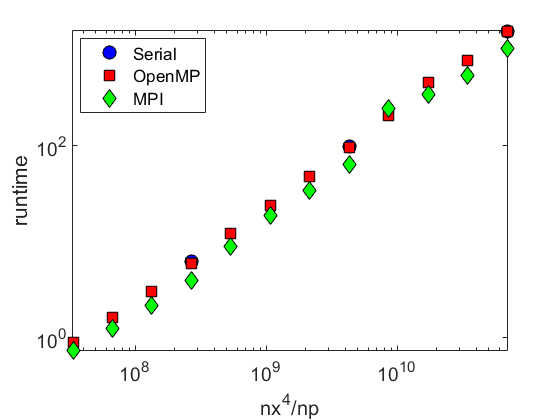
\includegraphics[width = \textwidth]{production2/scaling.png}
\end{figure} 

\section{Plots} 

Below are the final temperature distributions for each of the 30 required runs. Spatial units have been normalized by $\pi$. I apologize for the lousy figure placement. Wasn't worth fighting that battle in this case. 

% make the serial plots 
\foreach \nx in {128,256,512}{
\begin{figure}[htb]
\centering
\includegraphics[width = \textwidth]{{production2/out_serial.\nx}.png}
\end{figure} 
}

% make the omp plots 
\foreach \nx in {128,256,512}{
\foreach \np in {1,2,4,8} { 
\begin{figure}[htb]
\centering
\includegraphics[width = \textwidth]{{production2/out_omp.\nx .\np .all}.png}
\end{figure} 
}
}

% make the mpi plots 
\foreach \nx in {128,256,512}{
\foreach \np in {1,2,4,8,16} { 
\begin{figure}[htb]
\centering
\includegraphics[width = \textwidth]{{production2/out_mpi.\nx .\np .all}.png}
\end{figure} 
}
}

\section{Parallelization} 

For this assignment, it definitely took less time to modify the serial program with OpenMP than with MPI. Since all of the parallel work could easily be grouped together in this application, the code did not require substantial modifications or delicate reasoning to get working. Letting the compiler handle the details of the parallelization implicitly leaves less room for programming errors, and in fact, this was my experience. In contrast, I had several bugs during MPI development, some of which only appeared after I thought I had things working (\emph{e.g.} deadlocks that could be recovered from for small enough grids but were fatal for nx=512). However, with some experience, MPI feels more powerful, as explicitly programming the parallel instructions allows for more control. MPI also lifts the restriction of the number of processors to the total number on a node, which OpenMP must adhere to. Not only does this allow larger problem sizes to be solved, but theoretically it could also reduce queue wait times, as an MPI program could backfill the unused processors on partially used nodes, if such a scheme were implemented in a scheduler. 

For file I/O I used the same solution for OpenMP and MPI. Namely, each process writes to its own file, named in a systematic way: heat\_ $<$ method$>$ $<$nx$>$ $<$nprocs$>$ writes to heat\_ $<$method$>$.$<$nx$>$.$<$nprocs$>$.$<$rank$>$. After each file has been written, the rank 0 process uses a system call (cat) to concatenate the files together into heat\_ $<$method$>$.$<$nx$>$.$<$nprocs$>$.all, which contains all of the data. Since the domain decomposition is in order of rank, the data in each subfile preserves this order. This method of file I/O is suitable to this task because there are a relatively small (O(10)) number of independent processes which each have a potentially large amount of data. If this program were run with O(100)-O(1000) processors, the file I/O should be revisited. 
 
 \end{document}